
\chapter{ Compodoc }
Having a documentation tool within your app is incredibly important. The reason it's important, is that it increases visibility of your application in two areas in particular:
\begin{enumerate}
  \item Overview 
  \item Dependencies
  \item Various types of Modules, Components, Services etc. 
  \item Routes
  \item Documentation coverage
\end{enumerate}

Let's go through how to install compodoc, and the areas we have analyzed it is useful in, regarding documentation. 

\section{ Install Compodoc }
npm install -g @compodoc/compodoc --save-dev

\section{ Add a package.json script }
\begin{verbatim}
  "compodoc": "compodoc -p tsconfig.json",
  "compodoc-serve": "compodoc -s tsconfig.json",
\end{verbatim}

Now if we want to generate documentation, and we are in development mode, we can simply run 
\begin{verbatim}
npm run compodoc-serve  
\end{verbatim}

\section{Overview - Using Compodoc to Remove Dead Code}
Compodoc has a section called overview. It allows you to see all of your modules, components, and services. By doing so, you can see how they all feed into each other. 

\begin{figure}[h!]
\caption{Compodoc overview}
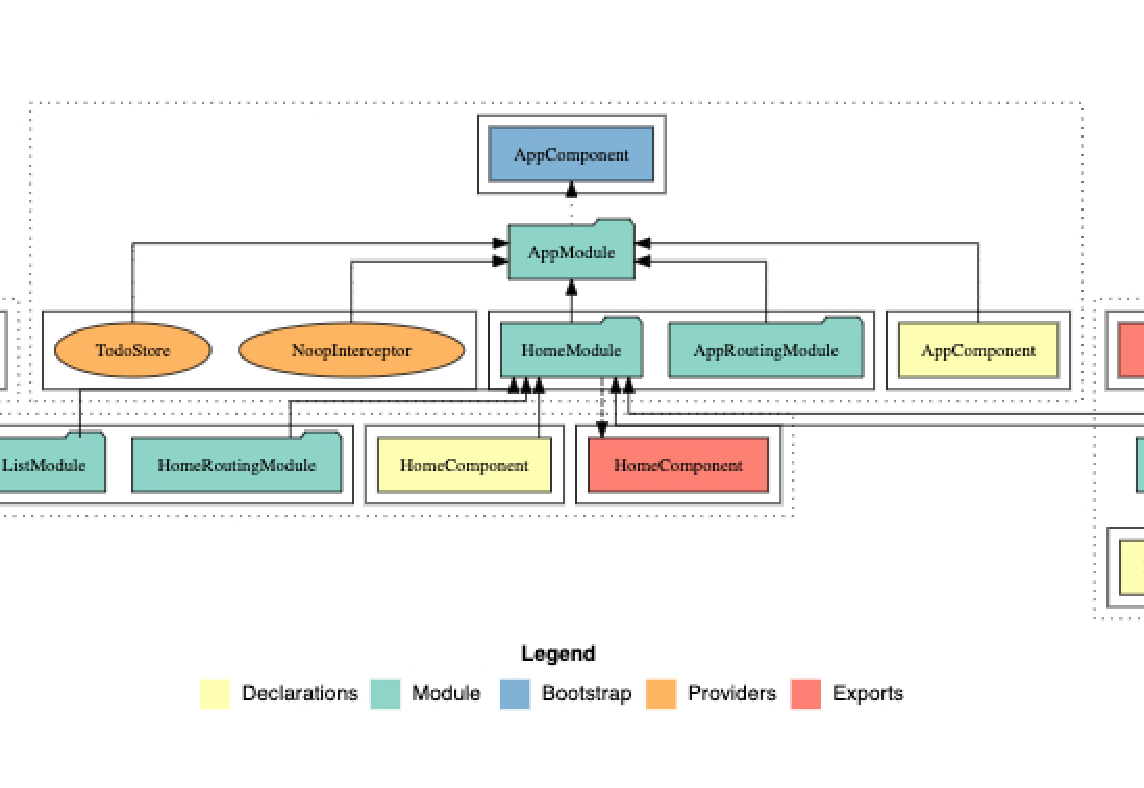
\includegraphics[width=414pt]{graphics/compodoc/compodoc-overview-screenshot.pdf}
\end{figure}

In the above image, we can see how Compodoc works. We can very clearly see what components are feeding into which module. If too many lines are randomly feeding into each other, then we know our app needs to be better organized. Also, if we have any components that do not feed into any modules, then we can clearly say that it is dead code, and should be deleted.

\section{Depedencies}
While it would be as simple as going into your package.json, it does stick out like a sore thumb, and does make you keep it in mind. So if this was the only feature, it wouldn't have that much value. However, I do like the fact that they did include it. 
\begin{figure}[h!]
\caption{Compodoc overview}
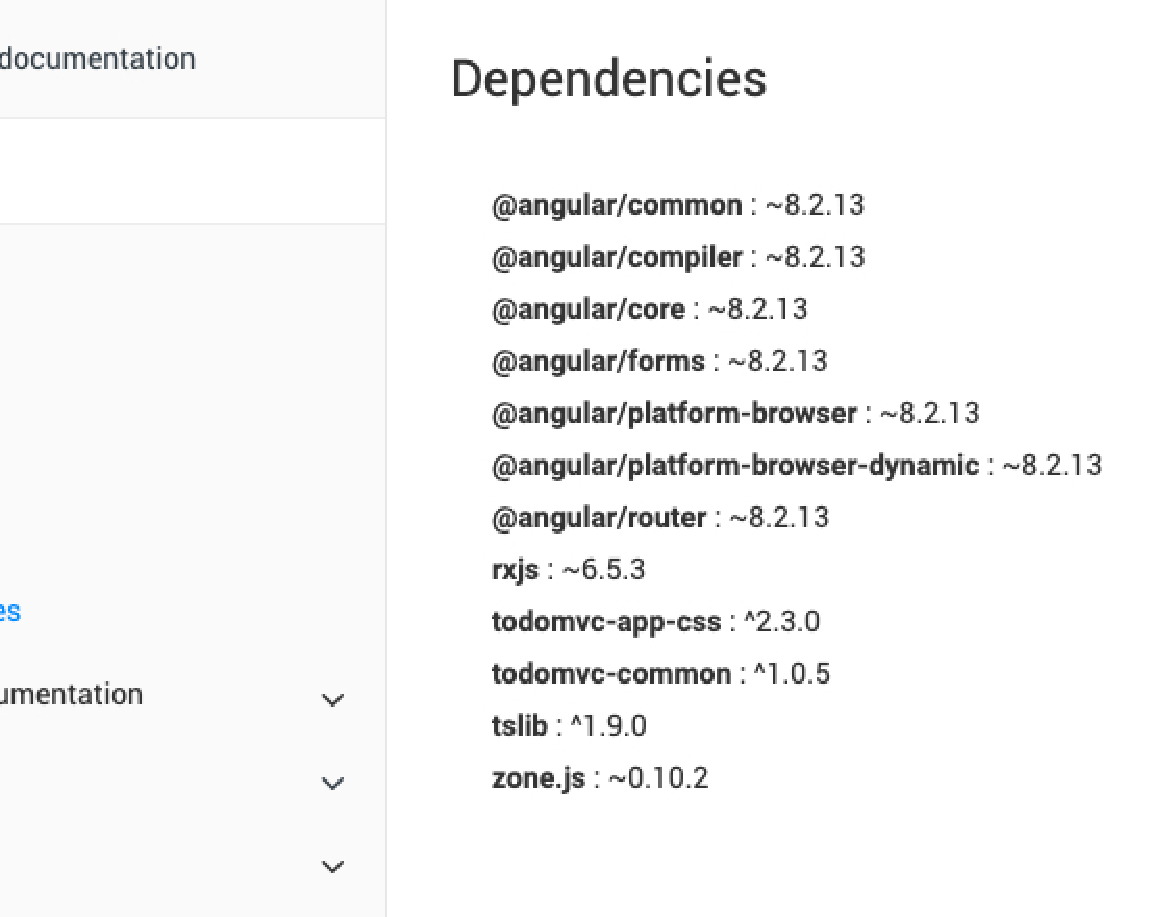
\includegraphics[width=414pt]{graphics/compodoc/dependencies/compo-dependencies-screenshot.pdf}
\end{figure}

So we can look through the above and immediately, oh ok, this is what version of angular we are on. I really like it for that reason, because the package.json has a way of creeping up on a project. This makes sure that it is front and center. 

\section{Various Types of Modules, Components etc.}
Compodoc also has offers dropdown of all modules, components, classes, services, interceptors, guards, interfaces, nad miscellaneous within app. I like this for two reasons: 
\begin{enumerate}
  \item It lays everything out there, so I know everything that's going on within my app.
  \item Also defines all the things that we should see in our app. In particular, I like the sections for interceptors, guards, and interfaces. It can leave an impact on the team, that these are things that should be written.
\end{enumerate}

\begin{figure}[h!]
\caption{Compodoc navigation of Modules, Components, etc.}
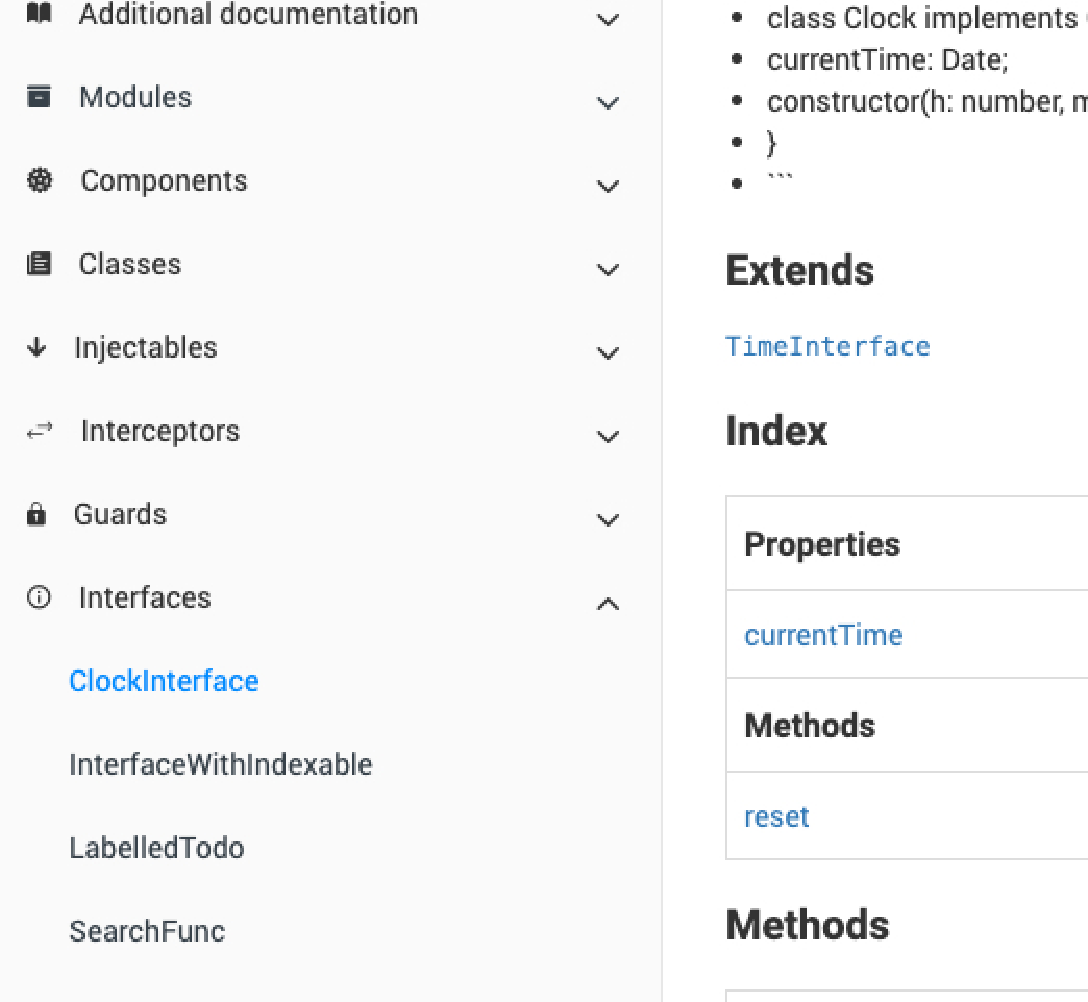
\includegraphics[width=414pt]{graphics/compodoc/nav/compodoc-nav-screenshot.pdf}
\end{figure}

\section{Routes}
Another one of the favorites is the ability to visualize all the routes that are in your application, and which components are attached. 

\begin{figure}[h!]
\caption{Compodoc Routes Example}
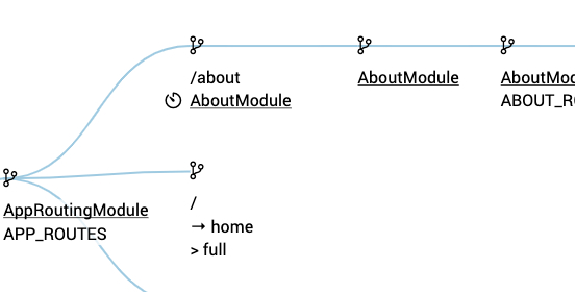
\includegraphics[width=414pt]{graphics/compodoc/routes/compodoc-routes.pdf}
\end{figure}

It also gives you the ability to click through the routes and see which components are using a particular route.

\section{Documentation Coverage}
Documentation coverage is another cool item with regards to compodoc. It's something that already exists in a number of different frameworks. However, it is nice that compodoc includes it, so all documentation is included in one place. In particular, the flavor of documentation it uses is JsDoc. For instance, if we have a method within our component, and it looks some like this: 
\begin{lstlisting}
/**
  * Display only completed todos
  */
displayCompleted() {
  this.currentFilter = 'completed';
  EmitterService.get(this.id).emit('displayCompleted');
}
/**
  * Display all todos
  */
displayAll() {
  this.currentFilter = 'all';
  EmitterService.get(this.id).emit('displayAll');
}
\end{lstlisting}

\begin{figure}[h!]
\caption{Compodoc Documentation Example}
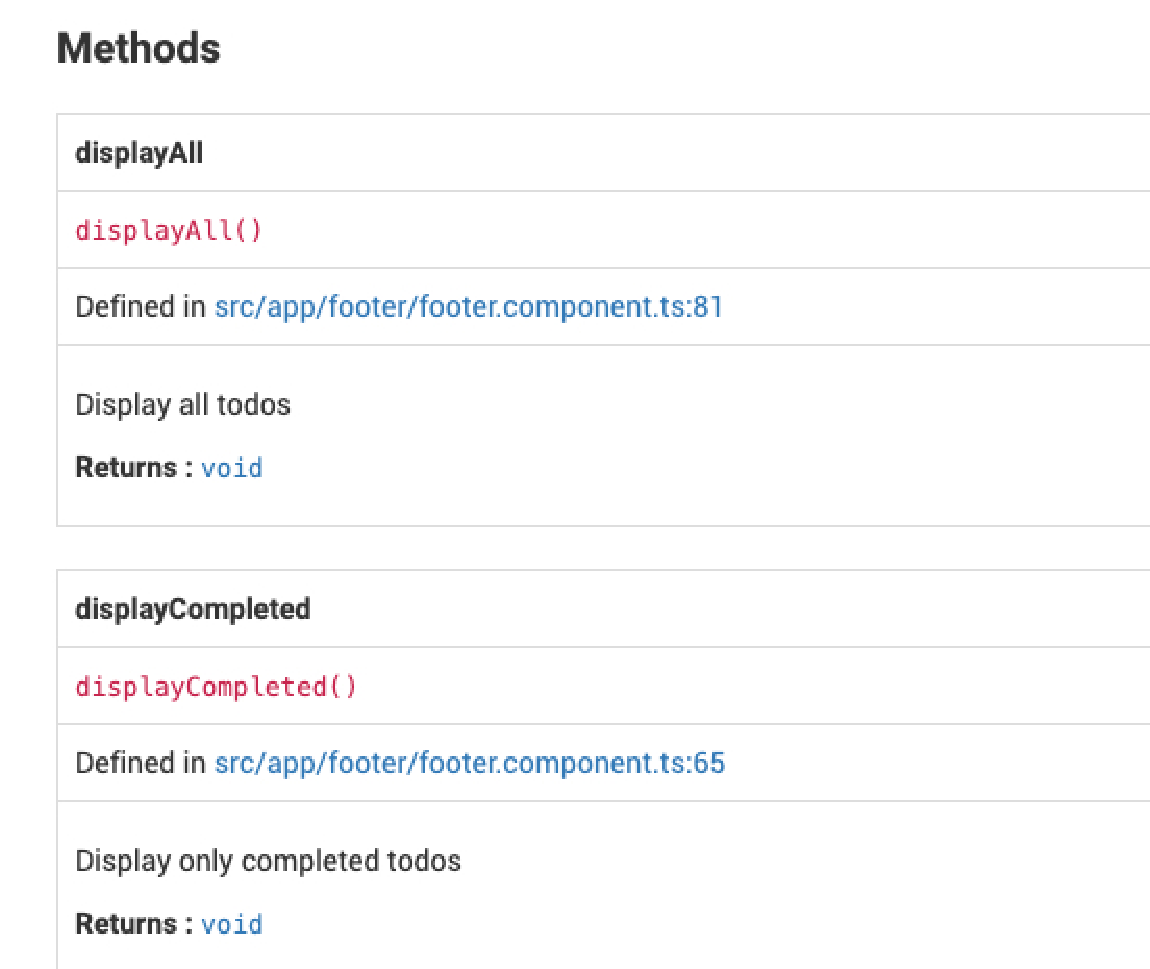
\includegraphics[width=414pt]{graphics/compodoc/documentation/documentation-coverage.pdf}
\end{figure}

It will take the JsDoc documentation and generate it in a way that is very, very easy to peruse. 